% Main rotation-curve figures for hybrid v3.3

\begin{figure}[h!]
\centering
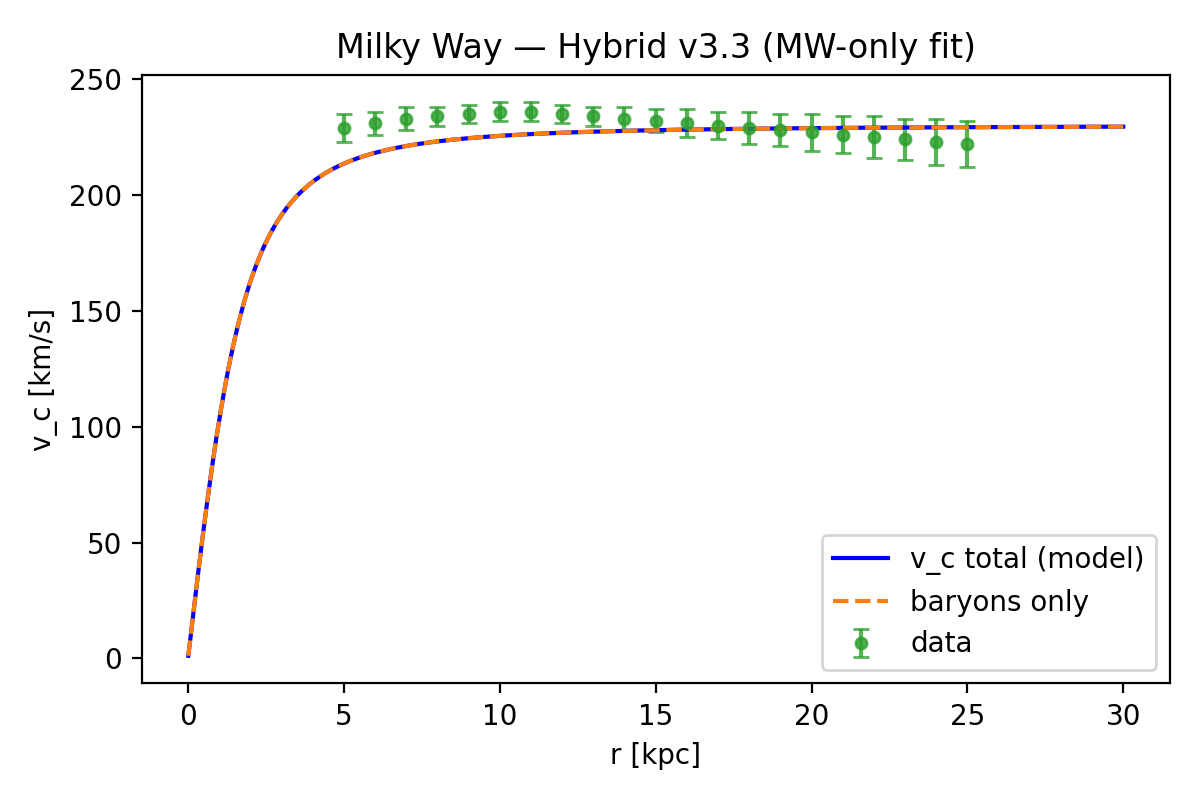
\includegraphics[width=0.7\textwidth]{mw_hybrid_v3_3_mw_only.png}
\caption{Milky Way rotation curve fit with the hybrid v3.3 model (MW-only fit).}
\label{fig:mw_hybrid_v33_mw_only}
\end{figure}

\begin{figure}[h!]
\centering
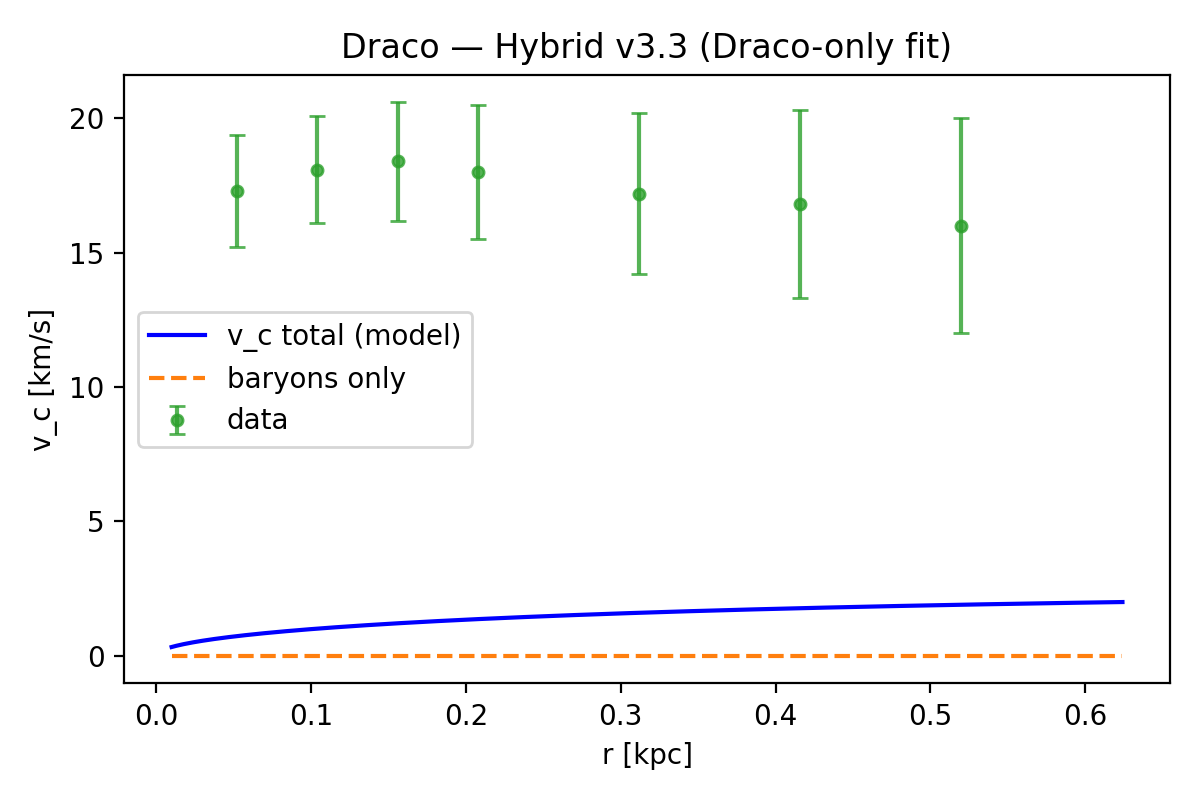
\includegraphics[width=0.7\textwidth]{draco_hybrid_v3_3_draco_only.png}
\caption{Draco rotation curve fit with the hybrid v3.3 model (Draco-only fit).}
\label{fig:draco_hybrid_v33_draco_only}
\end{figure}

\begin{figure}[h!]
\centering
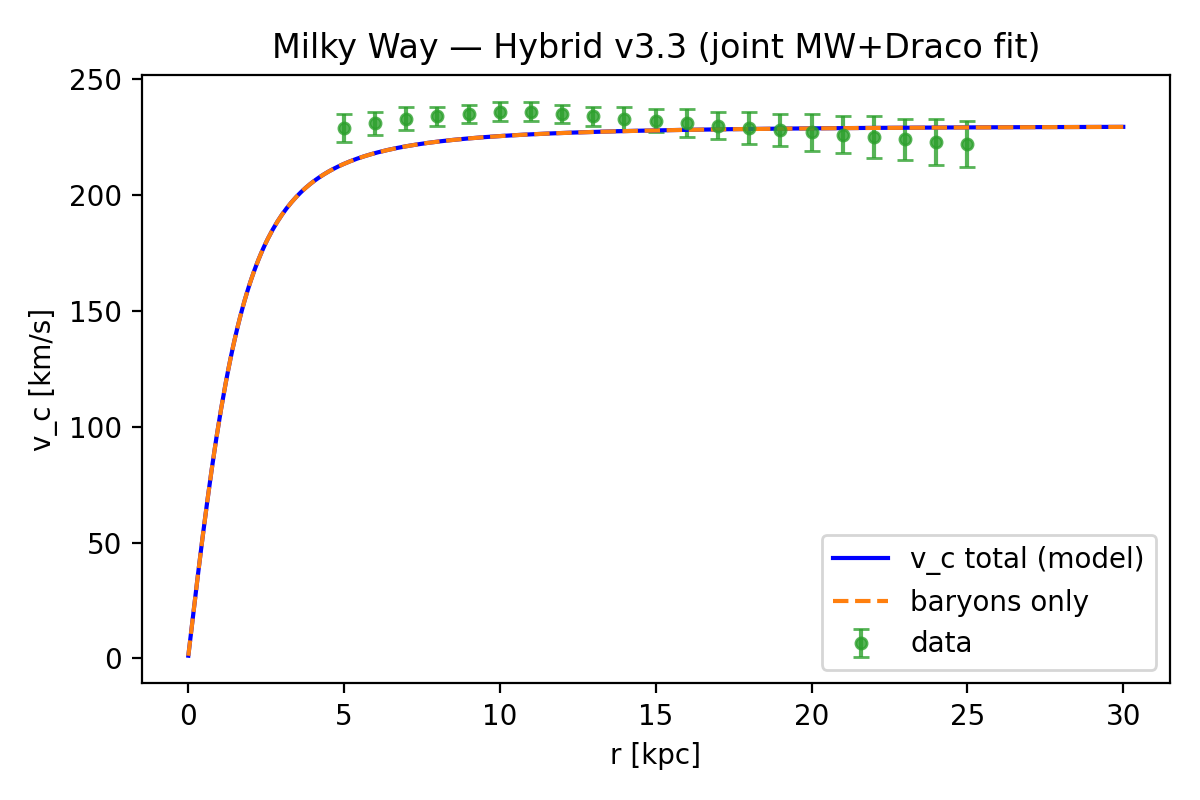
\includegraphics[width=0.48\textwidth]{mw_hybrid_v3_3_joint.png}
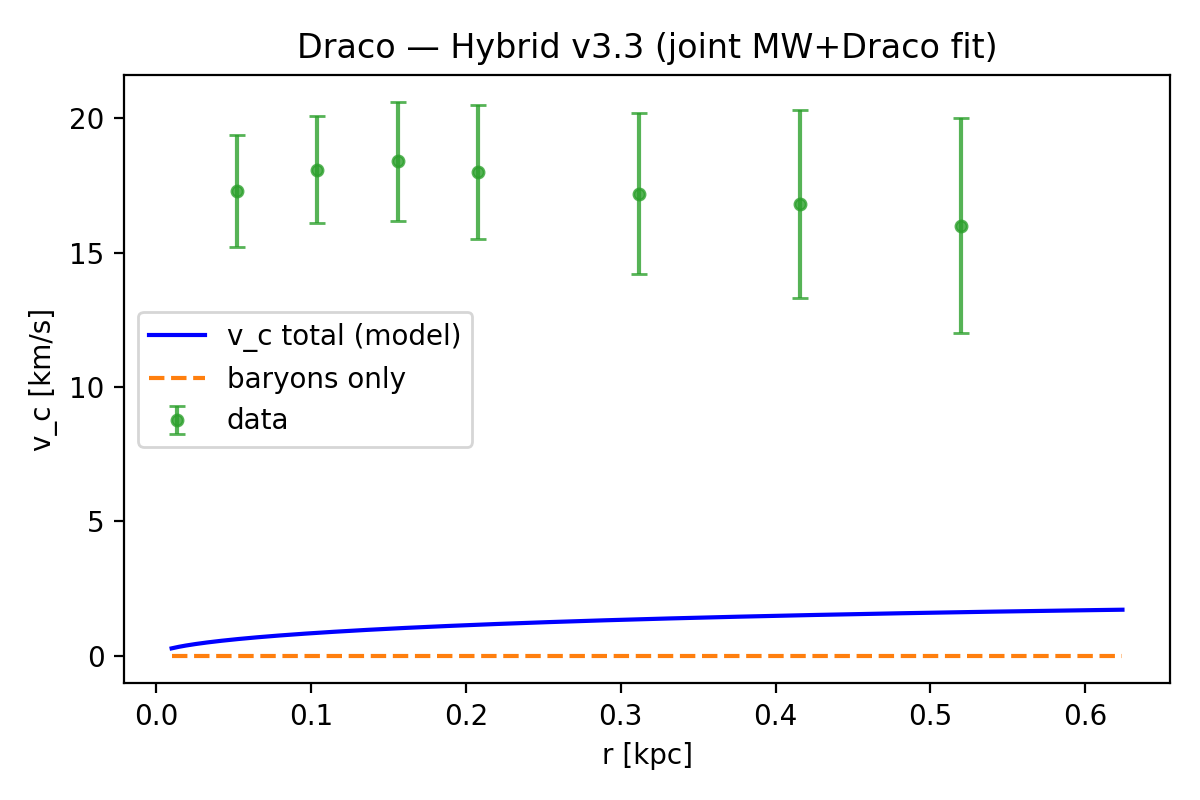
\includegraphics[width=0.48\textwidth]{draco_hybrid_v3_3_joint.png}
\caption{Joint hybrid v3.3 fit to the Milky Way (left) and Draco (right) rotation curves.}
\label{fig:mw_draco_hybrid_v33_joint}
\end{figure}

\begin{figure}[h!]
\centering
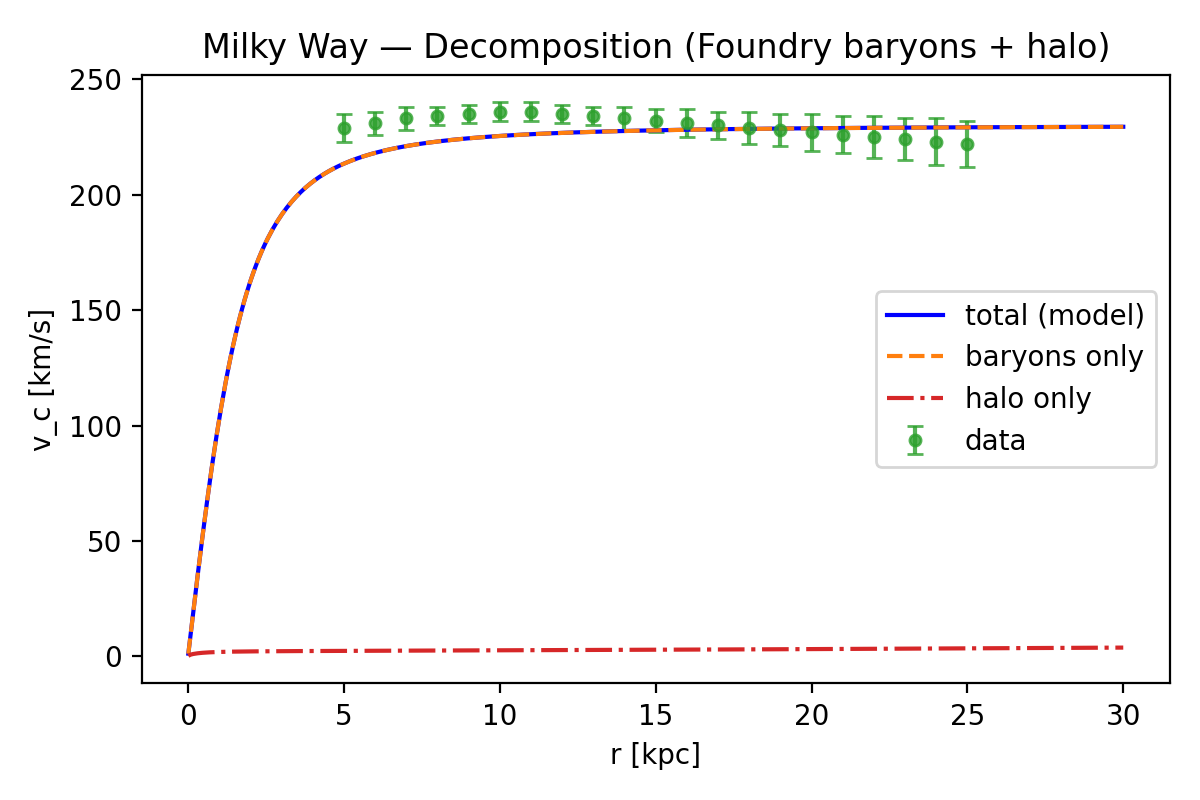
\includegraphics[width=0.48\textwidth]{mw_hybrid_v3_3_decomposition.png}
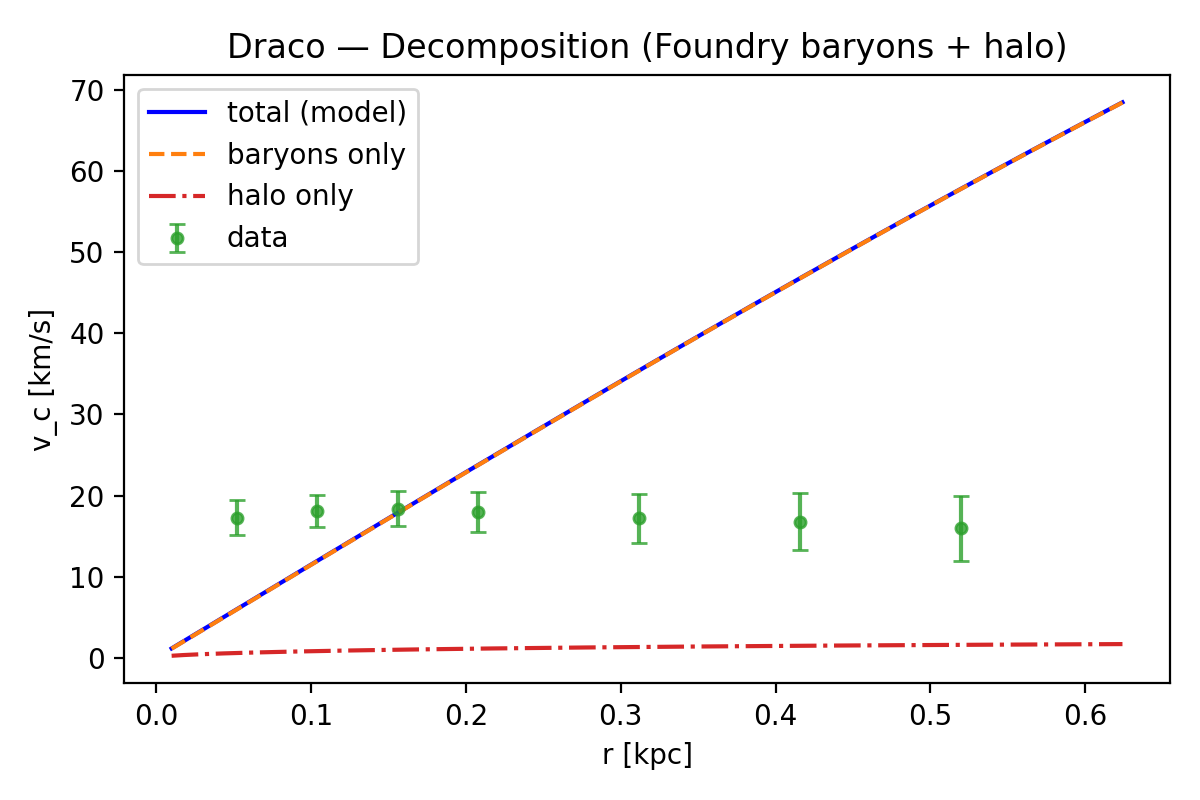
\includegraphics[width=0.48\textwidth]{draco_hybrid_v3_3_decomposition.png}
\caption{Decomposition of the hybrid v3.3 model into baryonic and halo components for the Milky Way (left) and Draco (right).}
\label{fig:mw_draco_hybrid_v33_decomposition}
\end{figure}

\begin{figure}[h!]
\centering
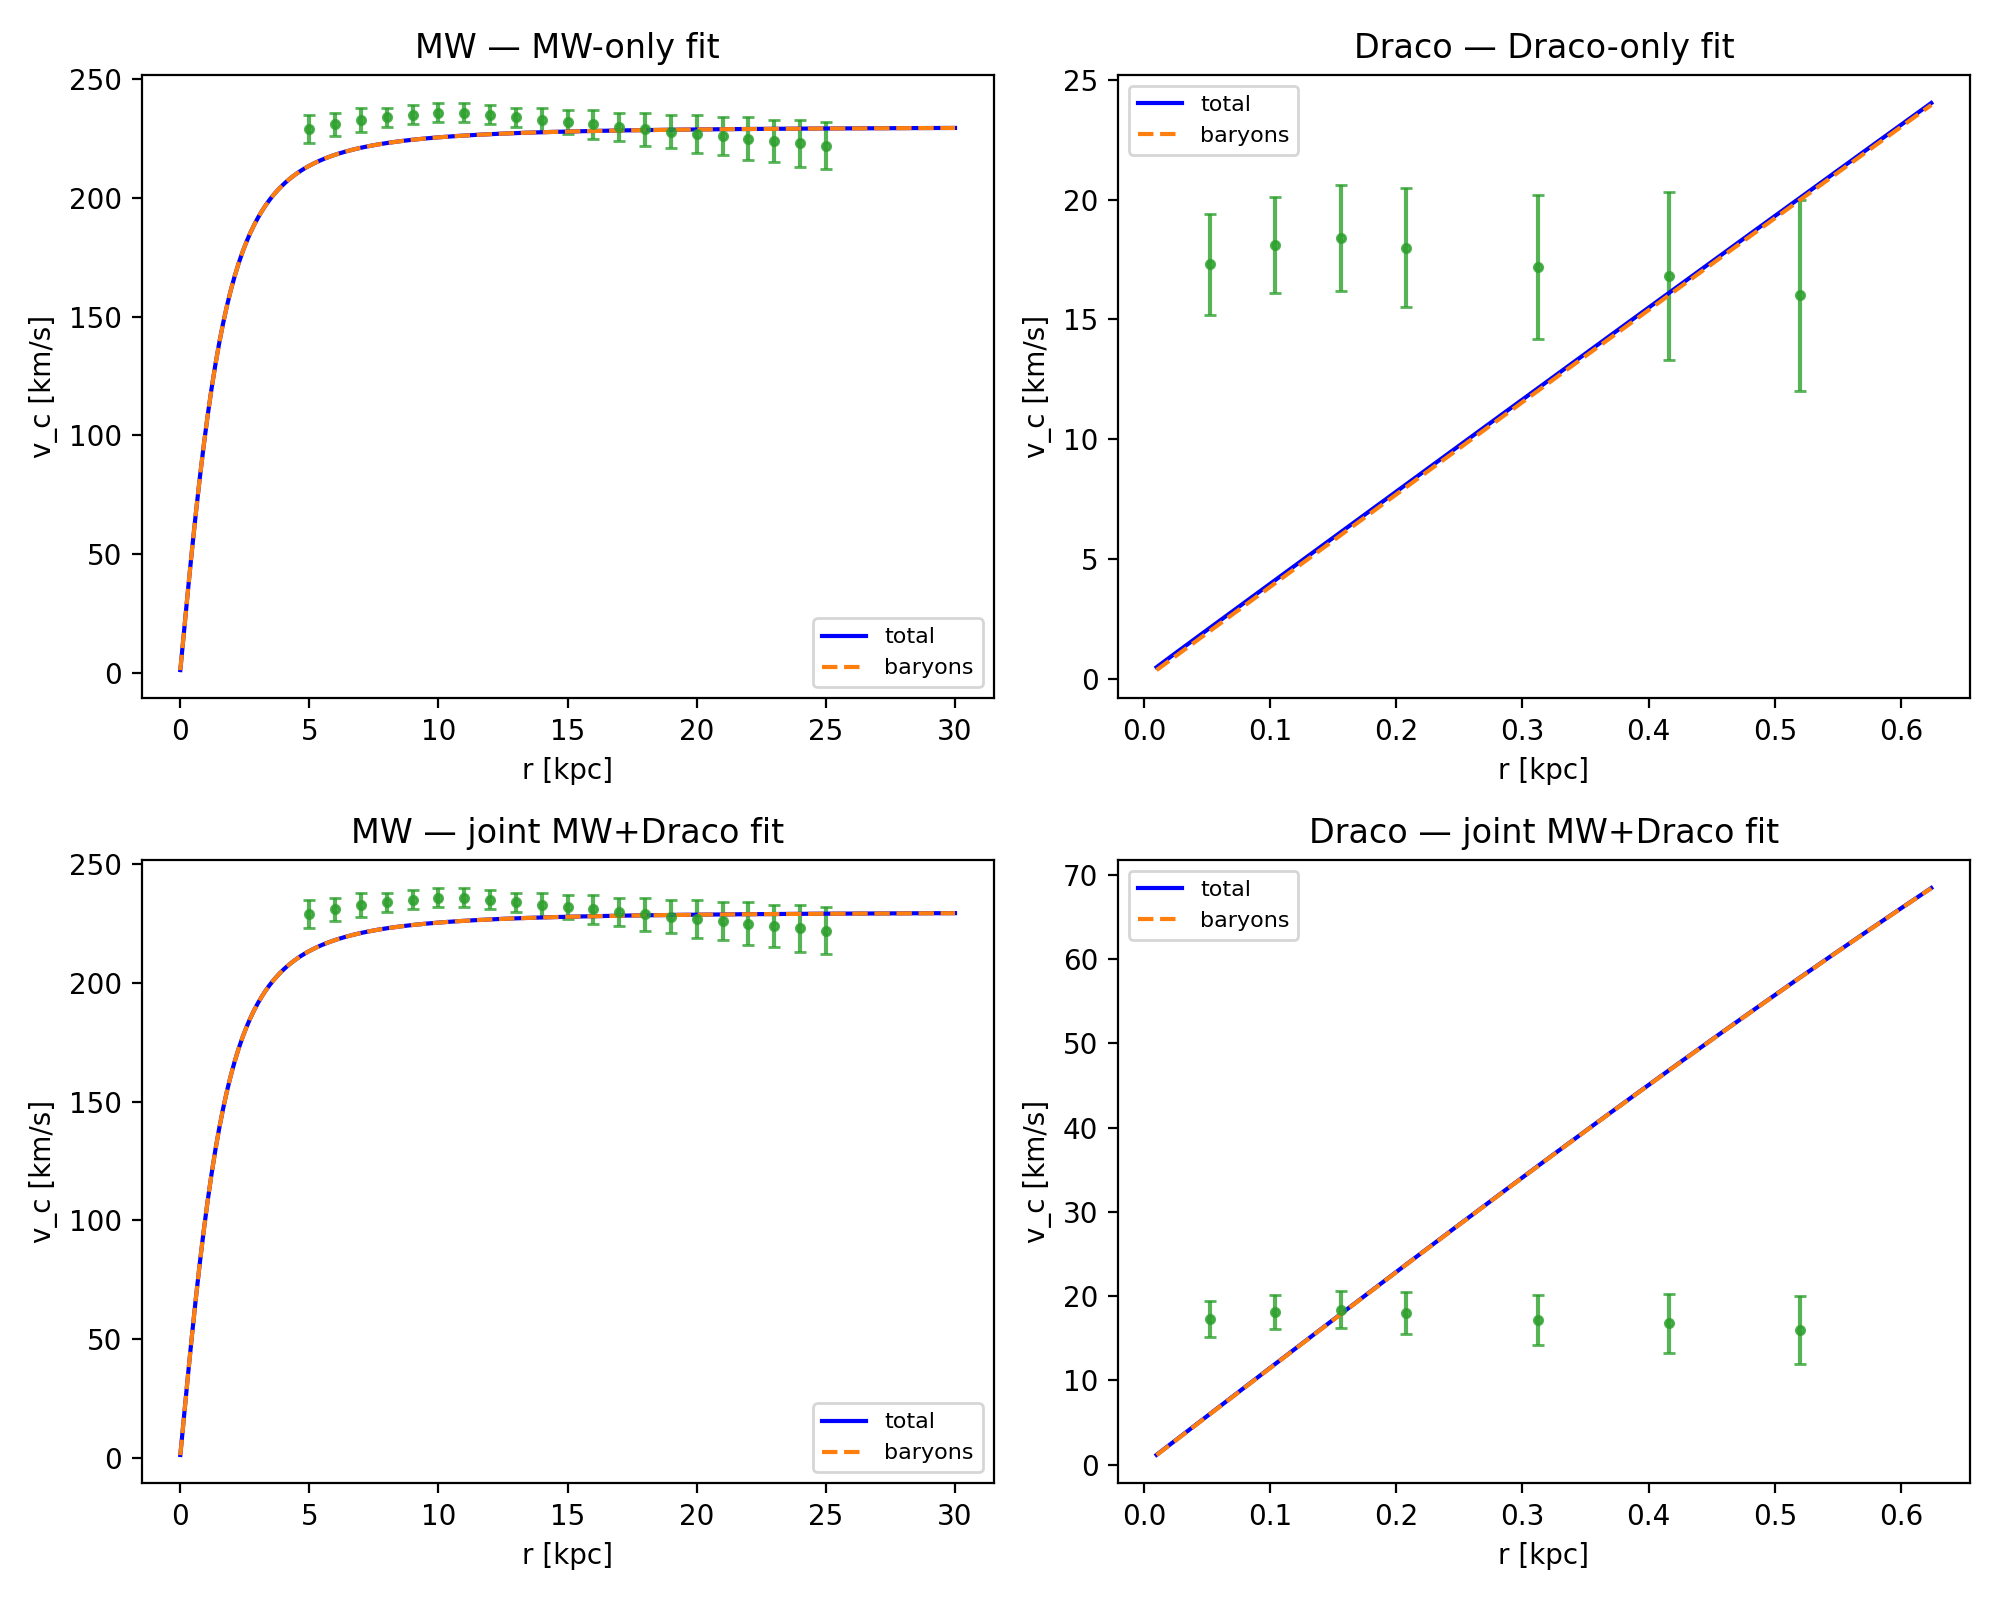
\includegraphics[width=0.9\textwidth]{hybrid_v3_3_summary_2x2.png}
\caption{Summary of hybrid v3.3 fits: MW-only, Draco-only, and joint MW+Draco fits in a 2�2 panel.}
\label{fig:hybrid_v33_summary_2x2}
\end{figure}
